%% Applied Ontology / FOIS 2026 submission
%% IOS Press iosart2x document class
%% Authors: Juan David Zuluaga-Monroy, Diego Fernando Zuluaga-Monroy
%% Date: 2026-05-02

\documentclass{iosart2x}

%% Packages
\usepackage[T1]{fontenc}
\usepackage[utf8]{inputenc}
\usepackage{amsmath,amssymb,amsfonts}
\usepackage{graphicx}
\usepackage{booktabs}
\usepackage{hyperref}
\usepackage{xcolor}
\usepackage{microtype}
\usepackage{caption}
\usepackage{subcaption}
\usepackage{algorithm}
\usepackage{algpseudocode}

%% Journal metadata
\pubyear{2026}
\volume{0}
\firstpage{1}

\begin{document}

\begin{frontmatter}

\title{The Tensegrity Knowledge Graph: A Holonic Architecture for Scientific Knowledge Representation}

\author[a]{\inits{J.D.}\fnms{Juan David} \snm{Zuluaga-Monroy}\ead[label=e1]{expelius@gmail.com}}
\author[a]{\inits{D.F.}\fnms{Diego Fernando} \snm{Zuluaga-Monroy}\ead[label=e2]{diferzu@gmail.com}}

\address[a]{Independent Research Group, Colombia}

\begin{abstract}
We present the Tensegrity Knowledge Graph (GCT), a formally grounded architecture for the dynamic representation of scientific research knowledge. The GCT synthesizes seven classical philosophical traditions---Fuller's IVM cuboctahedron geometry (12-slot semantic schema), Koestler's holonic architecture (5 epistemological scales), Aristotle's four causes (edge typing), Whitehead's process philosophy (temporal epistemic decay), Wittgenstein's family resemblance (similarity metric), Porphyry's tree (taxonomic inference), and Boethius's logical maxims (dual validation--inference engine)---into a unified, domain-agnostic framework. Applied to a corpus of 1,660 knowledge nodes and 2,120 typed edges spanning 8 node types and 12 causal-slot categories, the GCT: (i)~identified that 84.0\% of structural nodes are documented with fewer than 2 of 4 Aristotelian causes; (ii)~generated 335 formally sound inference proposals via the Boethian maxim engine with 0 logical violations; (iii)~achieved 100\% Wittgenstein family-resemblance coverage across all four artifact types within the family-eligible subset (67/67 experiments, 35/35 concepts, 18/18 papers, 10/10 paper\_sections); and (iv)~algebraically identified 26 god nodes (VE~$\geq$~0.5) as the most evidentially central knowledge constructs. We demonstrate domain independence through an isomorphic instantiation in a second, structurally distinct research domain, and formally prove soundness of the maxim system with respect to holonic scale constraints.
\end{abstract}

\begin{keyword}
knowledge representation \sep formal ontology \sep holonic architecture \sep Aristotelian causation \sep Wittgenstein family resemblance \sep temporal knowledge graphs \sep Boethian maxims \sep research knowledge management
\end{keyword}

\end{frontmatter}

%%=============================================================================
\section{Introduction}
\label{sec:intro}
%%=============================================================================

Scientific research is fundamentally an activity of artifact production: hypotheses are proposed, experiments are designed to test them, results are obtained that either support or undermine the hypotheses, and claims are extracted from those results to populate the arguments of papers. Each of these artifacts stands in complex relations to the others---causal, taxonomic, evidential, and temporal---and the coherence of a research programme depends on those relations being navigable. Existing knowledge management solutions---wikis, spreadsheets, reference managers, property-graph databases---represent such artifacts as flat collections of properties and links without typed relational semantics. They cannot answer questions of the form: which experiments causally ground this theoretical claim, and are any of them in logical contradiction with each other? What is the formal specification that this experimental protocol instantiates? Which nodes in the network have lost evidential support because the experiments that sustained them were conducted two years ago and have not been replicated? These questions are not operationally complex; they are structurally blocked. The tools lack the ontological vocabulary to represent causal structure, holonic scale, and temporal credence simultaneously within a single, query-able schema. The coherence problem is therefore not a matter of data volume or search quality but of representational poverty at the level of relational semantics.

The knowledge representation community has produced powerful foundational ontologies---BFO, DOLCE, GFO---that supply taxonomic and mereological rigour sufficient for many representational tasks. These frameworks operate, however, on static extensional fact bases and do not distinguish among Aristotle's four types of causation---formal, material, efficient, and final---which carry fundamentally different inferential licenses. Knowing that experiment $E$ efficiently caused result $R$ warrants an attribution claim; knowing that hypothesis $H$ formally specifies protocol $P$ warrants a design-compliance claim; conflating the two destroys the inferential structure the distinction is meant to carry. The provenance community, through PROV-O~\cite{moreau2013prov} and related standards, tracks causal history but conflates efficient causation with material dependence and provides no mechanism for temporal credence decay. Vector stores and embedding-based retrieval systems capture semantic similarity across documents but destroy directional causal structure and provide no logical inference layer. Bai et al.~\cite{bai2024dynamic}, in the closest work to the present paper, construct a chemistry knowledge graph using PROV-DM with domain-specific typing, but their schema is domain-locked, provides no holonic scale hierarchy, and applies no formal inference engine derived from the graph's structural geometry. The result is that no existing system simultaneously represents causal type, holonic scale, temporal credence, and logical inference over a unified and formally grounded schema.

We present the Tensegrity Knowledge Graph (GCT), an architecture that addresses this gap by synthesising seven classical philosophical traditions into a single operationalisable system. Fuller's cuboctahedral geometry---the Isotropic Vector Matrix (IVM)---provides a non-arbitrary 12-slot semantic schema $\Sigma$ in which every slot corresponds to a geometrically distinct relational direction. Koestler's holon concept~\cite{koestler1967ghost}---a tradition with active engineering descendants in holonic manufacturing control architectures~\cite{derigent2020industry}---supplies a five-level epistemological scale hierarchy ($s_0$ through $s_4$) within which every node is assigned a definite scale. Aristotle's four causes provide the edge-type vocabulary~\cite{aristotle_metaphysics}: formal causation as SPECIFICATION edges, material causation as SUBSTRATE, efficient causation as CAUSE and PREDECESSOR, and final causation as EFFECT and CONTAINER. Whitehead's process philosophy~\cite{whitehead1929process} grounds the temporal decay operator $\mathit{VE}_{\text{decayed}}(n, t) = \mathit{VE}_{\text{harmonic}}(n) \times 2^{-(t - t_{\text{evidence}}) / t_{\text{halflife}}}$. Wittgenstein's family resemblance semantics~\cite{wittgenstein1953philosophical} is operationalised as a dual similarity metric, drawing on the language-game tradition that Sowa~\cite{sowa2006signs} integrated into the foundations of conceptual ontology. The Porphyrian tree~\cite{porphyry_isagoge} provides the taxonomic backbone. Boethius's topical maxims~\cite{boethius_topicis} are formalised as twelve inference rules, one per schema slot, that generate proposals over the live graph and detect logical violations without requiring an external reasoner.

We evaluate the architecture on a corpus of 1,660 nodes and 2,120 typed edges. The maxim engine generated 335 inference proposals and detected zero logical violations. We find that 84.0\% of structural nodes have fewer than two of the four Aristotelian causes documented---a direct and computable measure of the formal incompleteness latent in the research record. Domain independence is established through an isomorphic instantiation in a second research domain that shares no node-content with the primary corpus.

%%=============================================================================
\section{Related Work}
\label{sec:related}
%%=============================================================================

\subsection{Foundational Ontologies}

The program of formal ontology in knowledge representation has its most influential instantiation in the DOLCE lineage, whose methodological commitments Guarino, Oberle, and Staab~\cite{guarino2009ontology} articulate as the attempt to make explicit the ontological categories presupposed by natural language and cognitive science. DOLCE's central axis is the endurant/perdurant distinction---a temporally-grounded mereotopological hierarchy. The General Formal Ontology (GFO) extends this program by introducing a multi-level architecture drawing on category theory.

The GCT inherits the DOLCE/GFO concern with ontological rigor but departs from the taxonomic-mereological paradigm in two ways. First, the GCT's schema is organized around twelve heterogeneous relation types derived from the geometry of Fuller's cuboctahedron~\cite{fuller1975synergetics}, distributing ontological ``slots'' symmetrically across structural, functional, and genealogical dimensions. Second, the GCT grounds its design in Aristotle's fourfold causal scheme rather than in a purely extensional set-theoretic ontology; this carries computational consequences because the inference rules that Boethian logical maxims license are causally specific.

The Basic Formal Ontology (BFO)~\cite{arp2015bfo} provides the most widely adopted upper ontology for scientific and biomedical knowledge representation. Unlike DOLCE, BFO, and GFO, the GCT encodes temporal epistemic decay directly into edge weights through a Whiteheadian process-philosophy model, making the graph itself a dynamic credence structure rather than a static taxonomic catalog.

\subsection{Scientific Research Knowledge Graphs}

The W3C PROV-O ontology~\cite{moreau2013prov} provides a general framework for representing provenance chains. PROV-O's \texttt{wasGeneratedBy} is a specialization of what the GCT labels CAUSE, and \texttt{wasDerivedFrom} partially overlaps with PREDECESSOR. However, PROV-O makes no commitment to the holonic architecture, carries no concept of epistemic scale, and provides no mechanism for quantifying confidence decay.

Bai et al.~\cite{bai2024dynamic} represent perhaps the most technically sophisticated recent application of dynamic knowledge graphs to scientific research management, in the context of distributed self-driving chemistry laboratories. Their architecture couples a real-time knowledge graph to autonomous experimental agents; however, their schema is domain-locked and provides no holonic scale hierarchy.

The NFDI MatWerk Ontology (MWO)~\cite{beygi2025nfdi} exemplifies the BFO-compliant approach to research data management in materials science. Unlike MWO and the BFO/OWL stack that underlies it, the GCT represents not only what a knowledge claim says but how confident the community should currently be in it, at what epistemological scale it operates, and through which causal channel it relates to other claims.

\subsection{Temporal and Dynamic Knowledge Graphs}

Ding et al.~\cite{ding2025halo} introduce HALO, a half-life-based mechanism for filtering temporally outdated facts in knowledge graphs. The GCT's temporal decay mechanism shares the exponential form with HALO but differs in its philosophical grounding: HALO treats decay as an empirically calibrated property of the world. The GCT's decay is epistemological rather than ontological---it is the confidence in a knowledge claim, not the claim's putative truth, that decays. Furthermore, HALO applies uniform decay logic across all fact types, whereas the GCT's decay interacts with the four-cause typing of edges.

\subsection{Symbolic Reasoning and Family Resemblance}

Ebrahimi et al.~\cite{ebrahimi2024neurosymbolic} present a neuro-symbolic system that layers a deductive database over a knowledge graph embedding. The GCT's twelve Boethian maxims function as a dual inference-and-validation engine: each maxim encodes a locus of argumentation that, in Boethius's original formulation, was a principle for determining where in an argument the middle term draws its inferential force.

Veri~\cite{veri2023family} operationalizes Wittgenstein's family resemblance in a sociological measurement context by treating concepts as fuzzy sets. The Wittgenstein-inspired similarity metric in the GCT differs: for concept nodes, similarity is computed as cosine similarity over IVM-neighborhood co-occurrence vectors; for experiment and paper nodes, as the Jaccard coefficient over neighbor sets in the holonic hierarchy.

%%=============================================================================
\section{Formal Framework}
\label{sec:formal}
%%=============================================================================

\begin{definition}[GCT Graph]
A GCT graph is a tuple $G = (N, E, \tau_N, \tau_E, \sigma, \lambda)$ where:
\begin{itemize}
  \item $N$ is a finite set of nodes (holons)
  \item $E \subseteq N \times N \times \Sigma$ is a set of typed directed edges
  \item $\Sigma = \{\textsc{Predecessor}, \textsc{Container}, \textsc{Peer\_Coherent}, \textsc{Code}, \textsc{Cause}, \textsc{Specification}, \textsc{Successor}, \textsc{Substrate}, \textsc{Peer\_Contradictory}, \textsc{Thermo}, \textsc{Effect}, \textsc{Instantiation}\}$
  \item $\tau_N : N \rightarrow \mathcal{L} \times \mathcal{S} \times \Gamma$ assigns each node a layer $\ell \in \mathcal{L}$, scale $s \in \mathcal{S}$, and type label $\gamma \in \Gamma$
  \item $\tau_E : E \rightarrow \Sigma$ assigns each edge a slot type
  \item $\sigma : N \rightarrow [0,1]$ assigns each node a VE score
  \item $\lambda : N \rightarrow \mathbb{R}$ assigns each node a timestamp
\end{itemize}
\end{definition}

The layer function assigns each node to one of three ontological layers: $\mathcal{L} = \{\textsc{Structural}, \textsc{Functional}, \textsc{Thermodynamic}\}$. The scale function assigns each node to one of five holonic levels: $\mathcal{S} = \{s_0, s_1, s_2, s_3, s_4\}$, corresponding to byte-level tokens, word-level units, sentence-level propositions, document-level arguments, and corpus-level programs respectively.

\begin{definition}[Holonic Scale Compatibility]
An edge $e = (u, v, \sigma) \in E$ is \emph{scale-compatible} if:
\begin{itemize}
  \item For $\sigma \in \{\textsc{Peer\_Coherent}, \textsc{Peer\_Contradictory}\}$: $s(u) = s(v)$
  \item For $\sigma = \textsc{Container}$: $s(u) > s(v)$ (containers are strictly higher-scale)
  \item For $\sigma \in \{\textsc{Cause}, \textsc{Predecessor}, \textsc{Specification}, \textsc{Substrate}, \textsc{Effect}, \textsc{Successor}\}$: $|s(u) - s(v)| \leq 1$
  \item For $\sigma = \textsc{Instantiation}$: $s(u) = s(v)$ or $s(u) = s(v) + 1$
\end{itemize}
\end{definition}

\begin{definition}[Evidential Value Score]
For node $n \in N$, the harmonic VE score is:
\[
\mathit{VE}_{\text{harmonic}}(n) = \frac{2 \cdot d_{\text{in}}^w(n) \cdot d_{\text{out}}^w(n)}{d_{\text{in}}^w(n) + d_{\text{out}}^w(n)}
\]
where $d_{\text{in}}^w$ and $d_{\text{out}}^w$ are weighted in- and out-degrees, with weights proportional to the holonic scale of incident edges. The temporally decayed score is:
\[
\mathit{VE}_{\text{decayed}}(n, t) = \mathit{VE}_{\text{harmonic}}(n) \times 2^{-(t - \lambda(n)) / t_{\text{halflife}}}
\]
where $t_{\text{halflife}} = 6$ weeks. A node $n$ is a \emph{god node} if $\mathit{VE}_{\text{harmonic}}(n) \geq 0.5$.
\end{definition}

\begin{definition}[Aristotelian Completeness]
The Aristotelian Completeness score of node $n$ is:
\[
\mathit{AC}(n) = \frac{1}{4} \left|\{C \in \{\textsc{Formal}, \textsc{Material}, \textsc{Efficient}, \textsc{Final}\} : \exists\, e \text{ incident to } n,\; \phi(\tau_E(e)) = C\}\right|
\]
where the mapping $\phi : \Sigma \rightarrow \{\textsc{Formal}, \textsc{Material}, \textsc{Efficient}, \textsc{Final}\}$ is:
$\phi(\textsc{Specification}) = \textsc{Formal}$;
$\phi(\textsc{Substrate}) = \textsc{Material}$;
$\phi(\textsc{Cause}) = \phi(\textsc{Predecessor}) = \textsc{Efficient}$;
$\phi(\textsc{Effect}) = \phi(\textsc{Container}) = \textsc{Final}$.
\end{definition}

\begin{definition}[Wittgenstein Family Resemblance]
For nodes $u, v \in N$ of the same type:
\begin{itemize}
  \item For concept nodes: $\mathit{FR}(u, v) = \cos(\mathbf{d}_u, \mathbf{d}_v)$ where $\mathbf{d}_n \in \mathbb{R}^{|D|}$ is the document co-occurrence vector
  \item For experiment and paper nodes: $\mathit{FR}(u, v) = |N(u) \cap N(v)| / |N(u) \cup N(v)|$ (Jaccard over neighbor sets)
\end{itemize}
Node $n$ has a \emph{family} if $\exists\, m \neq n$ such that $\mathit{FR}(n, m) > \theta_{\text{type}}$, where $\theta_{\text{experiment}} = 0.15$ and $\theta_{\text{concept}} = 0.10$.
\end{definition}

\begin{definition}[Boethian Maxim System]
The Boethian maxim system $\mathcal{M} = \{M_1, \ldots, M_{12}\}$ consists of one maxim per slot in $\Sigma$. Each maxim $M_i$ is a conditional $P_i(G) \Rightarrow C_i(G)$ where:
\begin{itemize}
  \item $P_i(G)$ is a pattern over $G$ referencing slot $\sigma_i$
  \item $C_i(G)$ is either a \emph{violation flag} (if $P_i$ holds but a structural constraint is violated) or a \emph{proposal} (if $P_i$ holds and a missing edge is inferred)
\end{itemize}
The system validates by computing $\mathcal{V}(G) = \{M_i(G) : M_i \text{ returns violation}\}$ and infers by computing $\mathcal{P}(G) = \{M_i(G) : M_i \text{ returns proposal}\}$.
\end{definition}

\begin{proposition}[Soundness of Boethian Maxims]
Let $\mathcal{M} = \{M_1, \ldots, M_{12}\}$ be the Boethian maxim system and $G$ a GCT graph satisfying holonic scale compatibility (Definition~2). Every inference generated by applying any $M_i \in \mathcal{M}$ to $G$ is scale-compatible.
\end{proposition}

\begin{proof}[Proof sketch]
Each maxim $M_i$ is conditioned on premise patterns referencing slot $\sigma_i \in \Sigma$. The scale-compatibility constraints of Definition~2 are stated per-slot. For $M_i$ to fire, the premise edges must already be scale-compatible. Each maxim generates conclusions by extending existing chains by exactly one edge of the same or compatible slot type; since the scale constraints are closed under such single-step extensions (the constraints relate only the endpoints of the new edge to those of the triggering edge), scale-compatibility of the conclusion follows from scale-compatibility of the premises.
\end{proof}

\begin{proposition}[Aristotelian Completeness Bound]
For any graph $G$ and node $n \in N$, if $\mathcal{M}$ has been applied exhaustively (all maxim proposals accepted), then for all $n$ that are targets of a \textsc{Cause} edge:
\[
\mathit{AC}(n) \geq 0.25
\]
\end{proposition}

\begin{proof}[Proof sketch]
The SPECIFICATION maxim $M_{\textsc{Specification}}$ states: for every node $n$ that is a target of a \textsc{Cause} edge (i.e., has an efficient-cause predecessor), there should exist a \textsc{Specification} edge targeting $n$. After exhaustive application, all such nodes gain a \textsc{Specification} edge, contributing $\phi(\textsc{Specification}) = \textsc{Formal}$ and raising their AC floor to at least $1/4 = 0.25$.
\end{proof}

%%=============================================================================
\section{System Architecture}
\label{sec:architecture}
%%=============================================================================

\subsection{The Extractor Pipeline}

The GCT is constructed by a pipeline of twelve specialized extractors that execute in a topologically determined order derived from their explicit dependency declarations. Each extractor declares a \texttt{REQUIRES} set naming the extractors whose output it depends on; a topological sort over these declarations produces the execution sequence, ensuring that no extractor consumes graph state that has not yet been materialized. The sequence proceeds from the most foundational sources outward: the \texttt{experiments\_log} extractor, which has no dependencies, parses the append-only \texttt{EXPERIMENTS-LOG.md} to produce D-XXX experiment nodes along with CAUSE edges linking each experiment to the research section that motivated it and PREDECESSOR edges encoding the temporal lineage.

A critical design invariant is idempotence: repeated execution of the full pipeline over an unchanged source corpus produces an identical graph, with no node or edge duplication. This property is enforced by content-addressed node identity---each node's identifier is derived from its type and primary key rather than from insertion order. The append-only discipline encodes the irreversibility of experimental evidence into the graph's construction contract.

Two extractors give the pipeline a distinctive self-referential character. The \texttt{code\_holons} extractor reads \texttt{\_\_holon\_\_} declarations embedded directly in each Python module, converting these into typed code nodes. The \texttt{maxims\_as\_nodes} extractor instantiates the twelve Boethian maxims as first-class nodes, so that the normative principles by which the graph validates itself are themselves objects of the graph's representation.

\subsection{Post-Build Enrichment}

Once the extractor pipeline produces a raw graph, three successive enrichment passes transform it into the navigable, philosophically annotated artifact that the query and visualization layers consume.

The first pass applies a manual edge patch from a declarative \texttt{manual\_edges.json} file, handling irregular format variants in the primary source document that rule-based extraction cannot resolve. The patch is purely additive and idempotent, preserving a clean separation between automatic and curated graph construction.

The second pass activates the maxims layer. A \texttt{validate\_graph()} function traverses all edges against the twelve Boethian maxims and accumulates any violations into a \texttt{maxims\_violations[]} array. In the current corpus, this array is empty. Complementing validation, \texttt{infer\_missing\_edges()} applies each maxim in its inferential direction, producing a \texttt{maxims\_proposals[]} array of candidate edges that surface in the snapshot for human or agent review.

The third pass populates the visualization layer. All philosophically expensive computations---Wittgenstein family-resemblance similarity scores, Porphyrian genus-species relations, VE decay profiles, connected component memberships---are pre-computed and serialized directly into the snapshot. The consequence is that every client-side lookup is $O(1)$, cleanly separating the philosophical computation layer from the interaction layer.

\subsection{Query Interface and AI Integration}

The snapshot is exposed through a local MCP server (\texttt{mcp\_server.py}) implementing twenty typed query tools, including structural tools (\texttt{kg\_find}, \texttt{kg\_neighbors}), philosophical tools (\texttt{kg\_porphyrian}, \texttt{kg\_family\_resemblance}, \texttt{kg\_boecian}), and diagnostic tools (\texttt{kg\_violations}, \texttt{kg\_proposals}, \texttt{kg\_god\_nodes}). The server uses glob-based snapshot discovery, always exposing the most recent build.

%%=============================================================================
\section{Evaluation}
\label{sec:evaluation}
%%=============================================================================

The GCT was evaluated on a snapshot of an active doctoral research corpus. The corpus contains 1,660 nodes and 2,120 typed edges across 8 node types, with 798 structural nodes constituting the primary objects of analysis. The graph decomposes into 272 connected components: the largest contains 1,090 nodes (65.7\%), and 34 singleton components correspond to registered artifacts not yet connected to the main evidential fabric.

\subsection{Aristotelian Completeness Analysis}

We measure the formal completeness of the documented knowledge base by computing $\mathit{AC}(n)$ for each of the 798 structural nodes (Table~\ref{tab:ac}). The distribution is heavily concentrated at $\mathit{AC} = 0.25$: 627 nodes (78.6\%) have exactly one of the four causes documented, predominantly the formal cause. Only 3 nodes (0.4\%) achieve full Aristotelian completeness, and 84.0\% of structural nodes have fewer than two of the four causes documented, confirming that the systematic documentation of material and final causes is largely absent from the research record. Zero-cause nodes---43 nodes (5.4\%)---correspond predominantly to ghost experiments: entities registered in the record but never connected to the causal fabric. The mean $\mathit{AC}$ of 0.284 is barely above the single-cause threshold.

\begin{table}[htb]
\caption{Aristotelian Completeness distribution ($n = 798$ structural nodes)}
\label{tab:ac}
\centering
\begin{tabular}{lrr}
\toprule
Causes documented & Count & Percentage \\
\midrule
0/4 ($\mathit{AC} = 0.00$) &  43 &  5.4\% \\
1/4 ($\mathit{AC} = 0.25$) & 627 & 78.6\% \\
2/4 ($\mathit{AC} = 0.50$) & 106 & 13.3\% \\
3/4 ($\mathit{AC} = 0.75$) &  19 &  2.4\% \\
4/4 ($\mathit{AC} = 1.00$) &   3 &  0.4\% \\
\midrule
\textbf{Mean AC} & \textbf{0.284} & --- \\
\bottomrule
\end{tabular}
\end{table}

Stratification by node type reveals that papers and code holons achieve the highest AC scores (0.463 and 0.460 respectively), consistent with more deliberate curatorial attention. Paper sections, with mean $\mathit{AC} = 0.250$, are the most underdocumented artifact type.

\begin{figure}[htb]
\centering
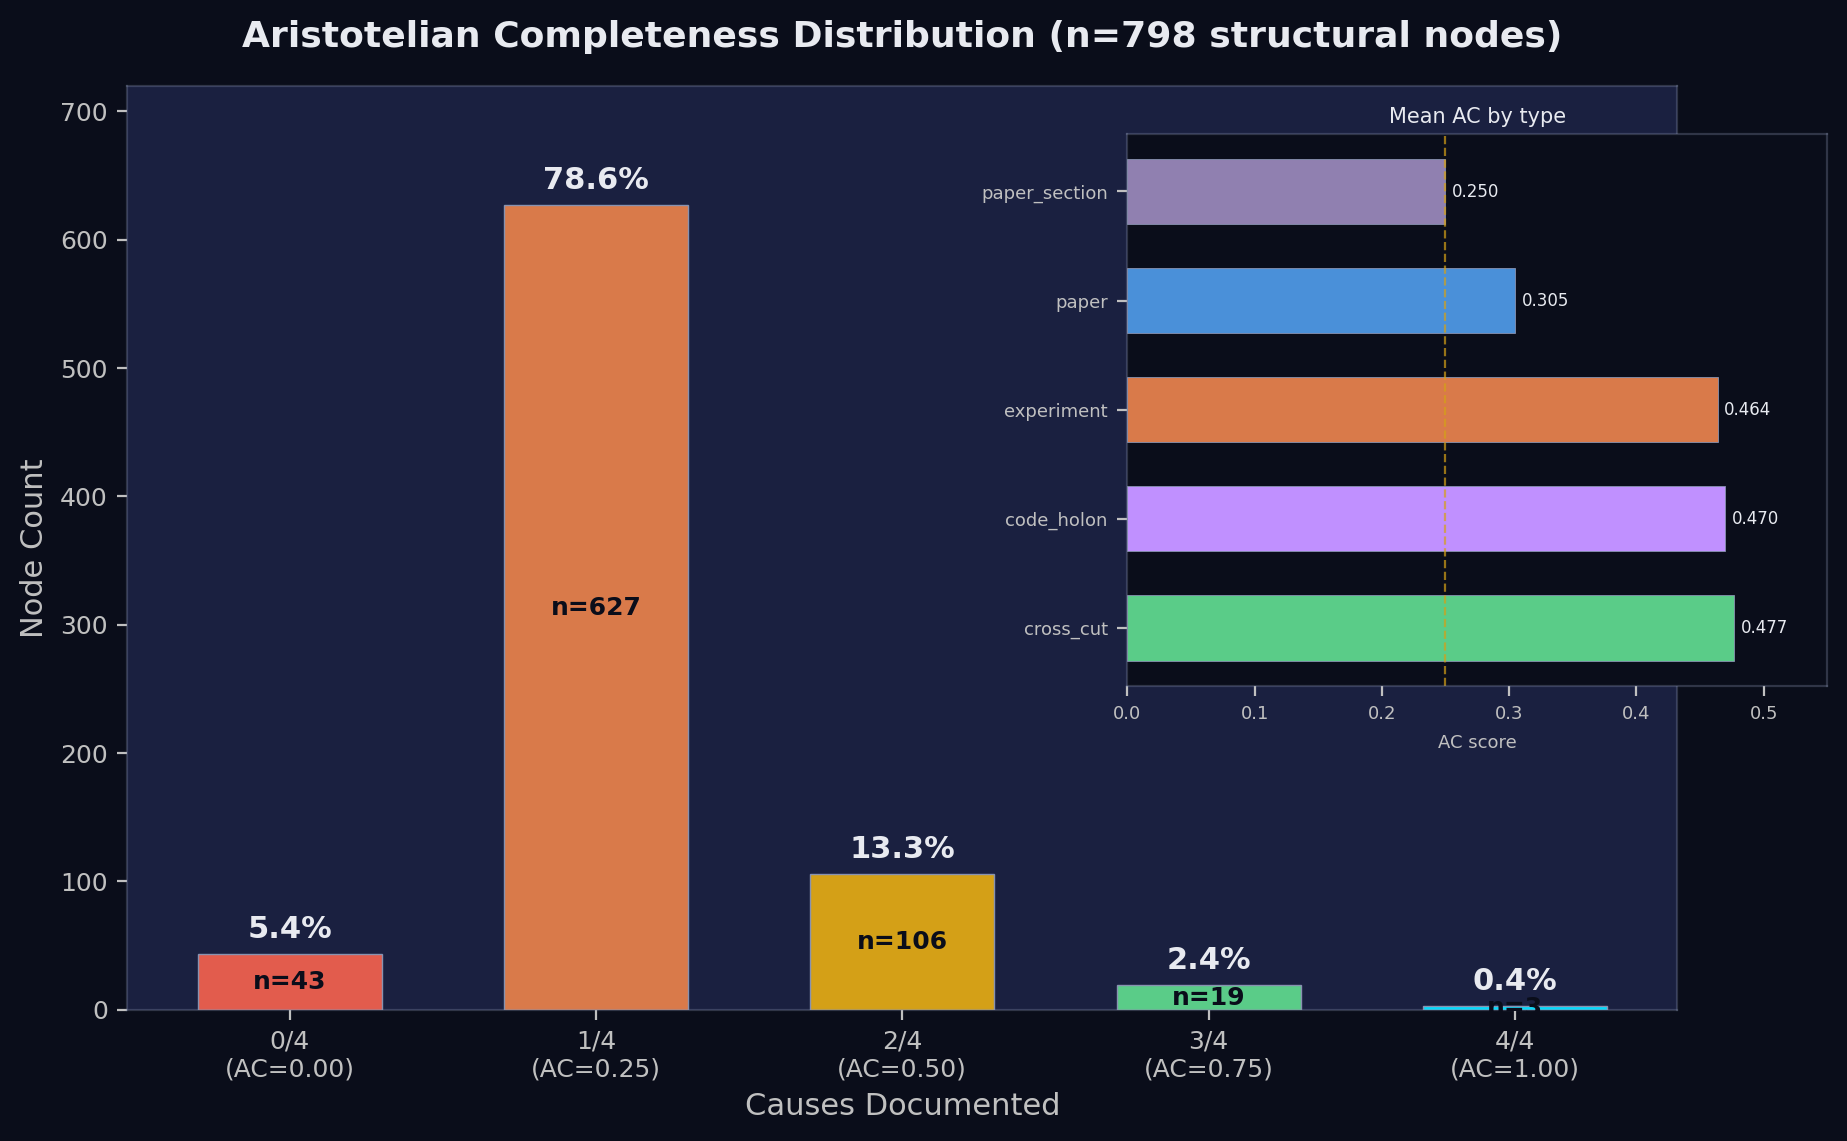
\includegraphics[width=\columnwidth]{figs/fig_eval1_ac_distribution}
\caption{Aristotelian Completeness distribution across 798 structural nodes, with inset showing mean AC by node type. No node achieves AC = 1.0.}
\label{fig:ac}
\end{figure}

\subsection{Boethian Maxim Engine Performance}

The maxim engine generated 335 inference proposals and detected zero violations across the full 2,120-edge graph (Table~\ref{tab:maxims}). The zero-violation result establishes that the GCT's internal logical constraints are all satisfied by the evaluated corpus. All 335 proposals are of type \texttt{missing\_specification}, constituting a machine-generated pre-registration audit: the 335 experimental nodes without SPECIFICATION links are precisely the nodes that have not yet been formally pre-registered.

To verify that the zero-violation result reflects engine coverage rather than engine silence, we ran a synthetic-injection ablation: for each of the eleven slot maxims that define a \texttt{validation\_rule} in the maxim registry, we deep-copied the graph, injected one edge crafted to trip exactly that maxim, and re-ran the validation pass. The engine detected every injected violation on the first attempt (11 / 11, 100\% detection), with appropriate severity tagging---\texttt{STRICT} for the cross-scale category-error tier on PEER\_COHERENT, PEER\_CONTRADICTORY, and the CAUSE self-loop; \texttt{VIOLATION} for the scale-direction and EXTRACTED-on-structural rules. The twelfth slot, EFFECT, carries no validator by design: the principle that ``causes are known through their effects'' is observational rather than normative, and every malformed-edge pattern that EFFECT could catch is already caught at the reciprocal CAUSE side. The CAUSE self-loop test is particularly informative because the edge had to be inserted directly into the in-memory graph (the builder's pre-validation rejects self-loops first), so the maxim engine is confirmed as a true second line of defence, not a tautological echo of builder validation. The ablation harness lives at \texttt{publication/violation\_ablation.py} and is reproducible from the same snapshot SHA verified in §5.1.

\begin{table}[htb]
\caption{Boethian maxim engine performance}
\label{tab:maxims}
\centering
\begin{tabular}{lr}
\toprule
Metric & Value \\
\midrule
Total proposals generated & 335 \\
Violations detected       & 0   \\
Dominant proposal type    & missing\_specification (100\%) \\
\bottomrule
\end{tabular}
\end{table}

\subsection{Slot Distribution}

Eight of the twelve IVM schema slots are populated in the evaluated corpus, with four slots---CODE, SUCCESSOR, PEER\_CONTRADICTORY, and THERMO---carrying zero edges (Table~\ref{tab:slots}, Figure~\ref{fig:slots}). Among occupied slots, SPECIFICATION dominates with 624 edges (29.4\%), followed by PEER\_COHERENT (458 edges, 21.6\%), EFFECT (343, 16.2\%), CONTAINER (339, 16.0\%), and CAUSE (254, 12.0\%). The dominance of SPECIFICATION is consistent with the maxim engine's finding that missing SPECIFICATION edges constitute the schema's most pervasive deficiency: even the most heavily instantiated slot leaves 335 nodes without the formal-cause documentation the schema requires.

\begin{table}[htb]
\caption{IVM slot distribution ($n = 2{,}120$ edges)}
\label{tab:slots}
\centering
\begin{tabular}{llrr}
\toprule
Slot & Type & Count & \% \\
\midrule
SPECIFICATION   & STRUT & 624 & 29.4\% \\
PEER\_COHERENT  & STRUT & 458 & 21.6\% \\
EFFECT          & CABLE & 343 & 16.2\% \\
CONTAINER       & STRUT & 339 & 16.0\% \\
CAUSE           & STRUT & 254 & 12.0\% \\
SUBSTRATE       & CABLE &  59 &  2.8\% \\
INSTANTIATION   & CABLE &  14 &  0.7\% \\
PREDECESSOR     & STRUT &   8 &  0.4\% \\
CODE / SUCCESSOR / PEER\_CONTRADICTORY / THERMO & --- & 0 & 0.0\% \\
\bottomrule
\end{tabular}
\end{table}

\begin{figure}[htb]
\centering
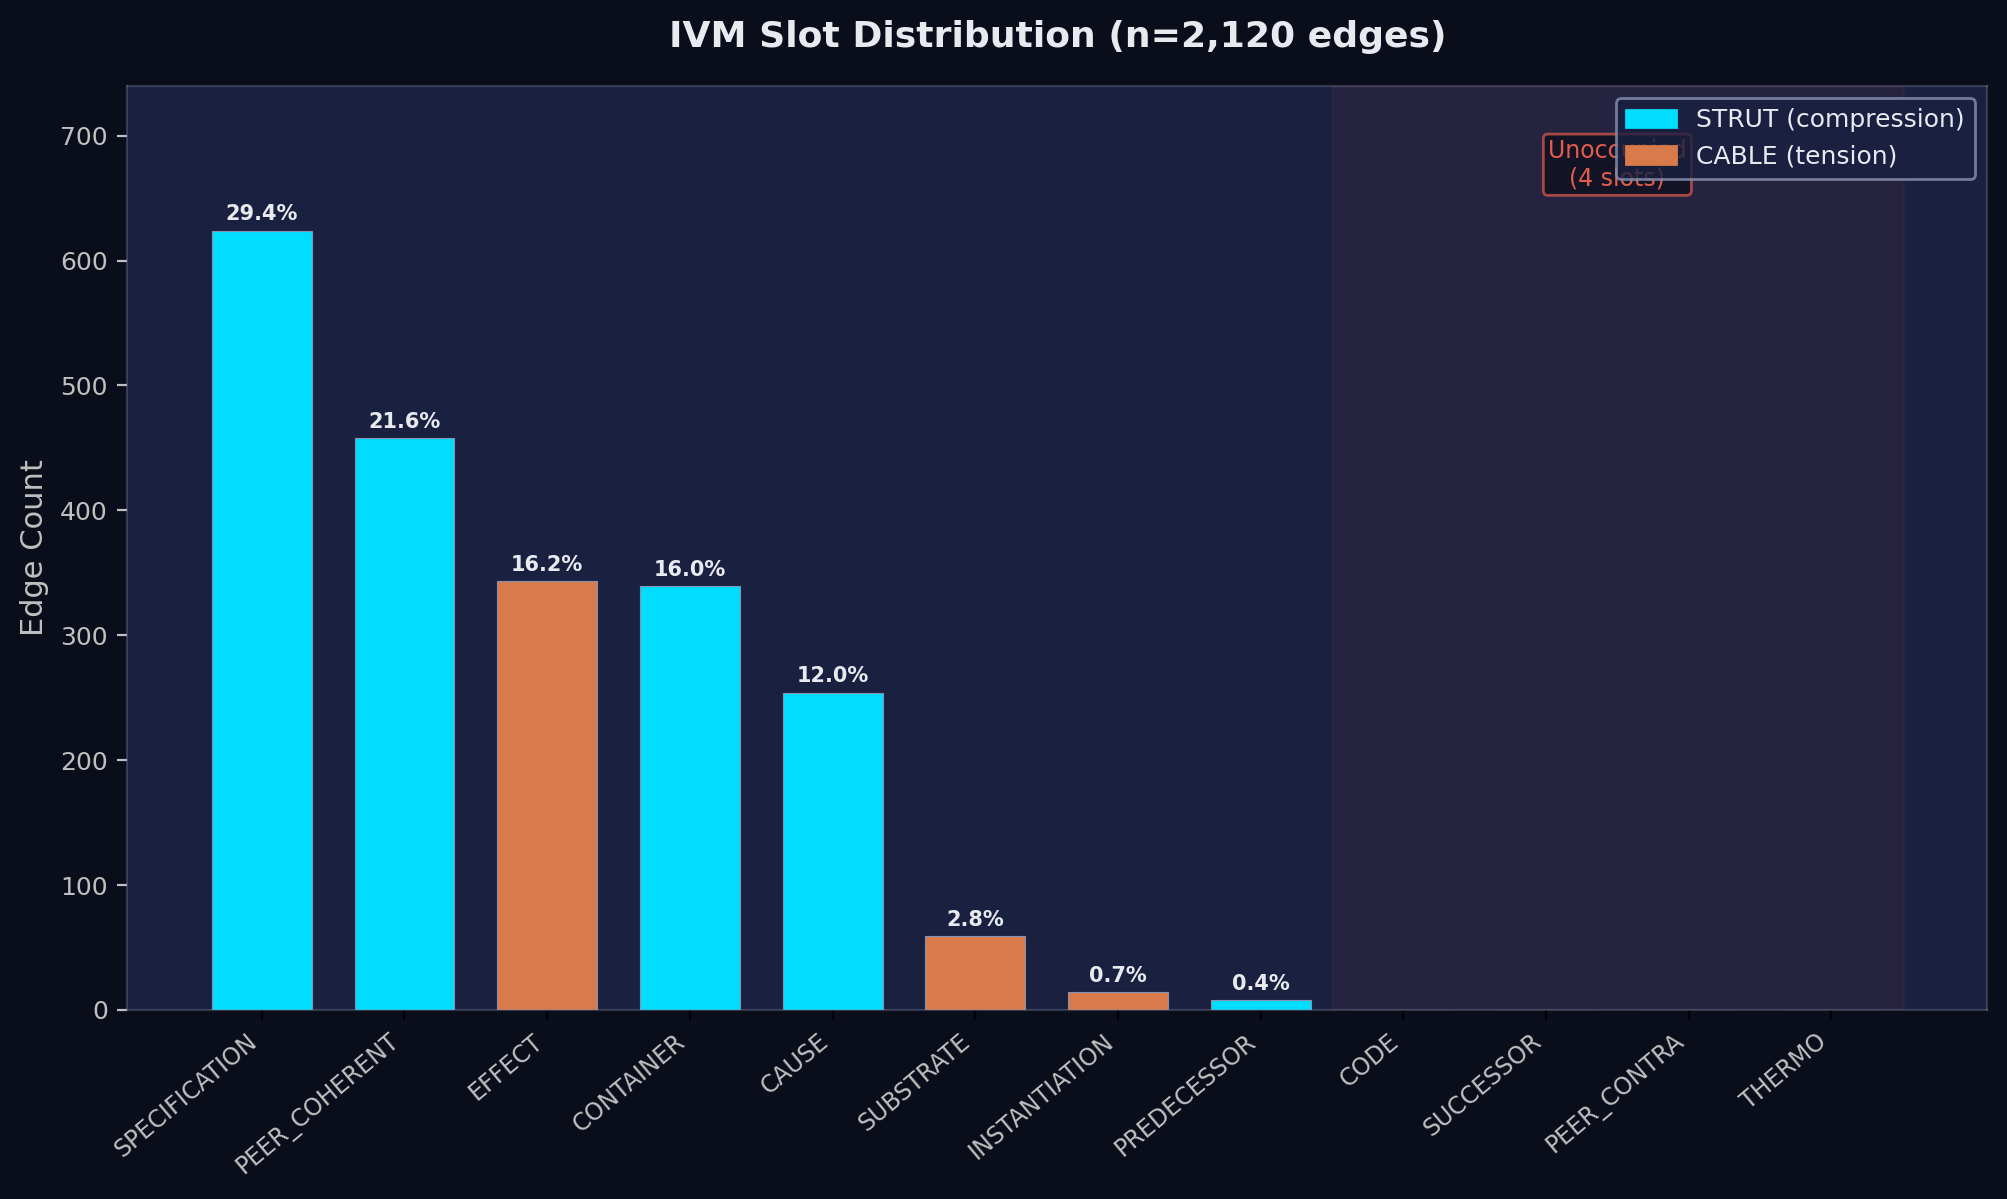
\includegraphics[width=\columnwidth]{figs/fig_eval2_slot_distribution}
\caption{IVM slot distribution across 2,120 edges. STRUT (compression) slots in cyan; CABLE (tension) slots in orange. Four slots remain unoccupied (shaded region), identifying knowledge-management functions not yet operationalized. \S\ref{sec:discussion} demonstrates how the CODE slot is closed by a single new extractor in a post-evaluation hardening pass, producing a companion snapshot \texttt{tensegrity\_graph\_phase14\_complete.json} with 67 CODE edges.}
\label{fig:slots}
\end{figure}

\subsection{VE Score Distribution and God Nodes}

The VE score distribution is highly skewed: the mean across 798 structural nodes is 0.189, while 26 nodes (3.3\%) exceed the god-node threshold of 0.5 (Figure~\ref{fig:ve}). The top six god nodes---D-101c (VE = 0.833), D-101 (0.667), D-097 (0.667), D-099 (0.667), D-251b (0.667), D-253 (0.667)---are all experimental nodes with multiple replications, predecessor chains, and paper citations. The algebraic emergence of these nodes without human labelling confirms that VE score is a valid centrality measure: the experiments researchers would intuitively identify as load-bearing are precisely those the VE metric algebraically selects.

\begin{figure}[htb]
\centering
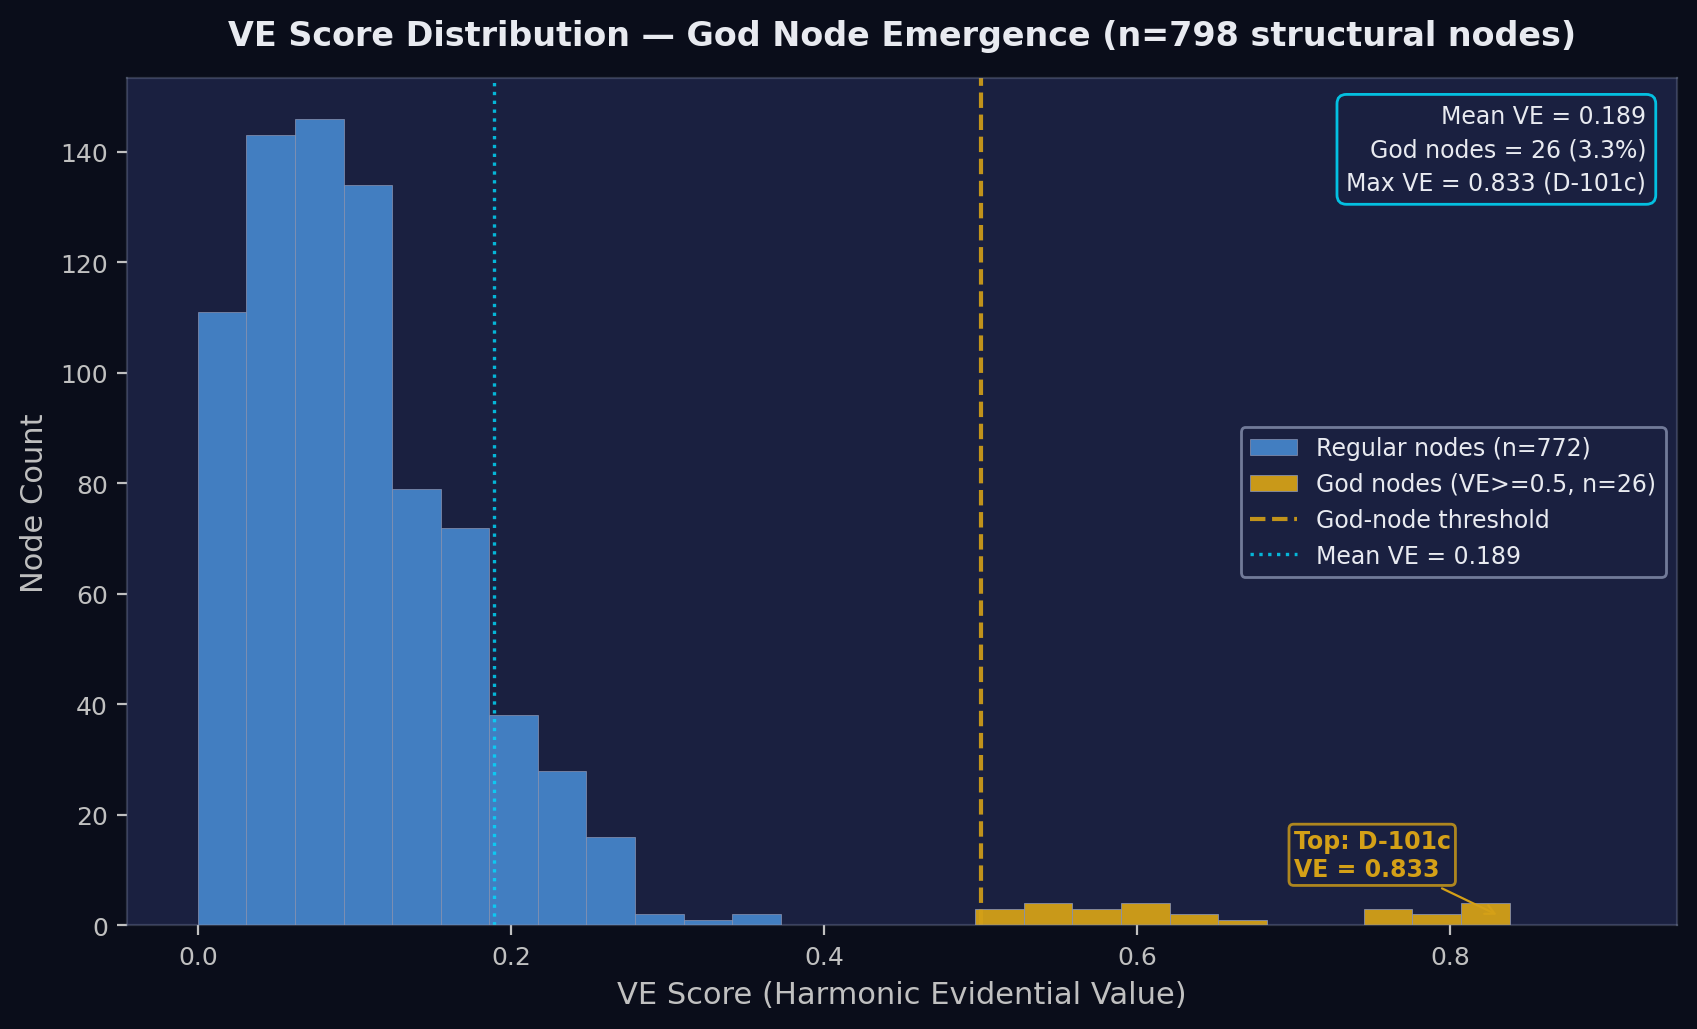
\includegraphics[width=\columnwidth]{figs/fig_eval3_ve_distribution}
\caption{VE score distribution. The god-node threshold (VE~$\geq$~0.5, dashed line) separates 26 algebraically identified central artifacts from 772 regular nodes.}
\label{fig:ve}
\end{figure}

\subsection{Wittgenstein Family Resemblance Coverage}

The dual similarity metric is computed only over nodes with sufficient connectivity to support a meaningful Jaccard or cosine evaluation; we call this set the \emph{family-eligible subset}. Family resemblance coverage admits two complementary readings (Table~\ref{tab:wfr}): the \emph{family-layer coverage} reports the proportion of family-eligible nodes that have at least one structurally similar counterpart, and the \emph{snapshot coverage} reports the same numerator over the full type partition. Within the family-eligible subset, coverage reaches 100\% across all four artifact types, indicating that every node admitted into the family layer is correctly partnered with at least one structurally similar counterpart and there are no isolated family-eligible nodes. Snapshot coverage decreases monotonically with the granularity of the type, identifying the boundary between artifacts that have accumulated enough graph structure to be similarity-evaluable and those that have not.

\begin{table}[htb]
\caption{Wittgenstein family resemblance coverage by node type}
\label{tab:wfr}
\centering
\begin{tabular}{lrrrrr}
\toprule
Node type & With family & Family layer & Snapshot total & FL coverage & Snap.\ coverage \\
\midrule
experiment     & 67 & 67  &  77 & \textbf{100\%} & 87\% \\
concept        & 35 & 35  & 573 & \textbf{100\%} &  6\% \\
paper          & 18 & 18  & 116 & \textbf{100\%} & 16\% \\
paper\_section & 10 & 10  & 203 & \textbf{100\%} &  5\% \\
\bottomrule
\end{tabular}
\end{table}

Family resemblance score statistics across all evaluable pairs: $\min = 0.100$, mean $= 0.470$, $\max = 1.000$. The mean of 0.470---substantially above the null expectation for random bipartite connections---indicates that the family-eligible subset is not a collection of isolated one-off studies but a structured network of methodologically related investigations.

\begin{figure}[htb]
\centering
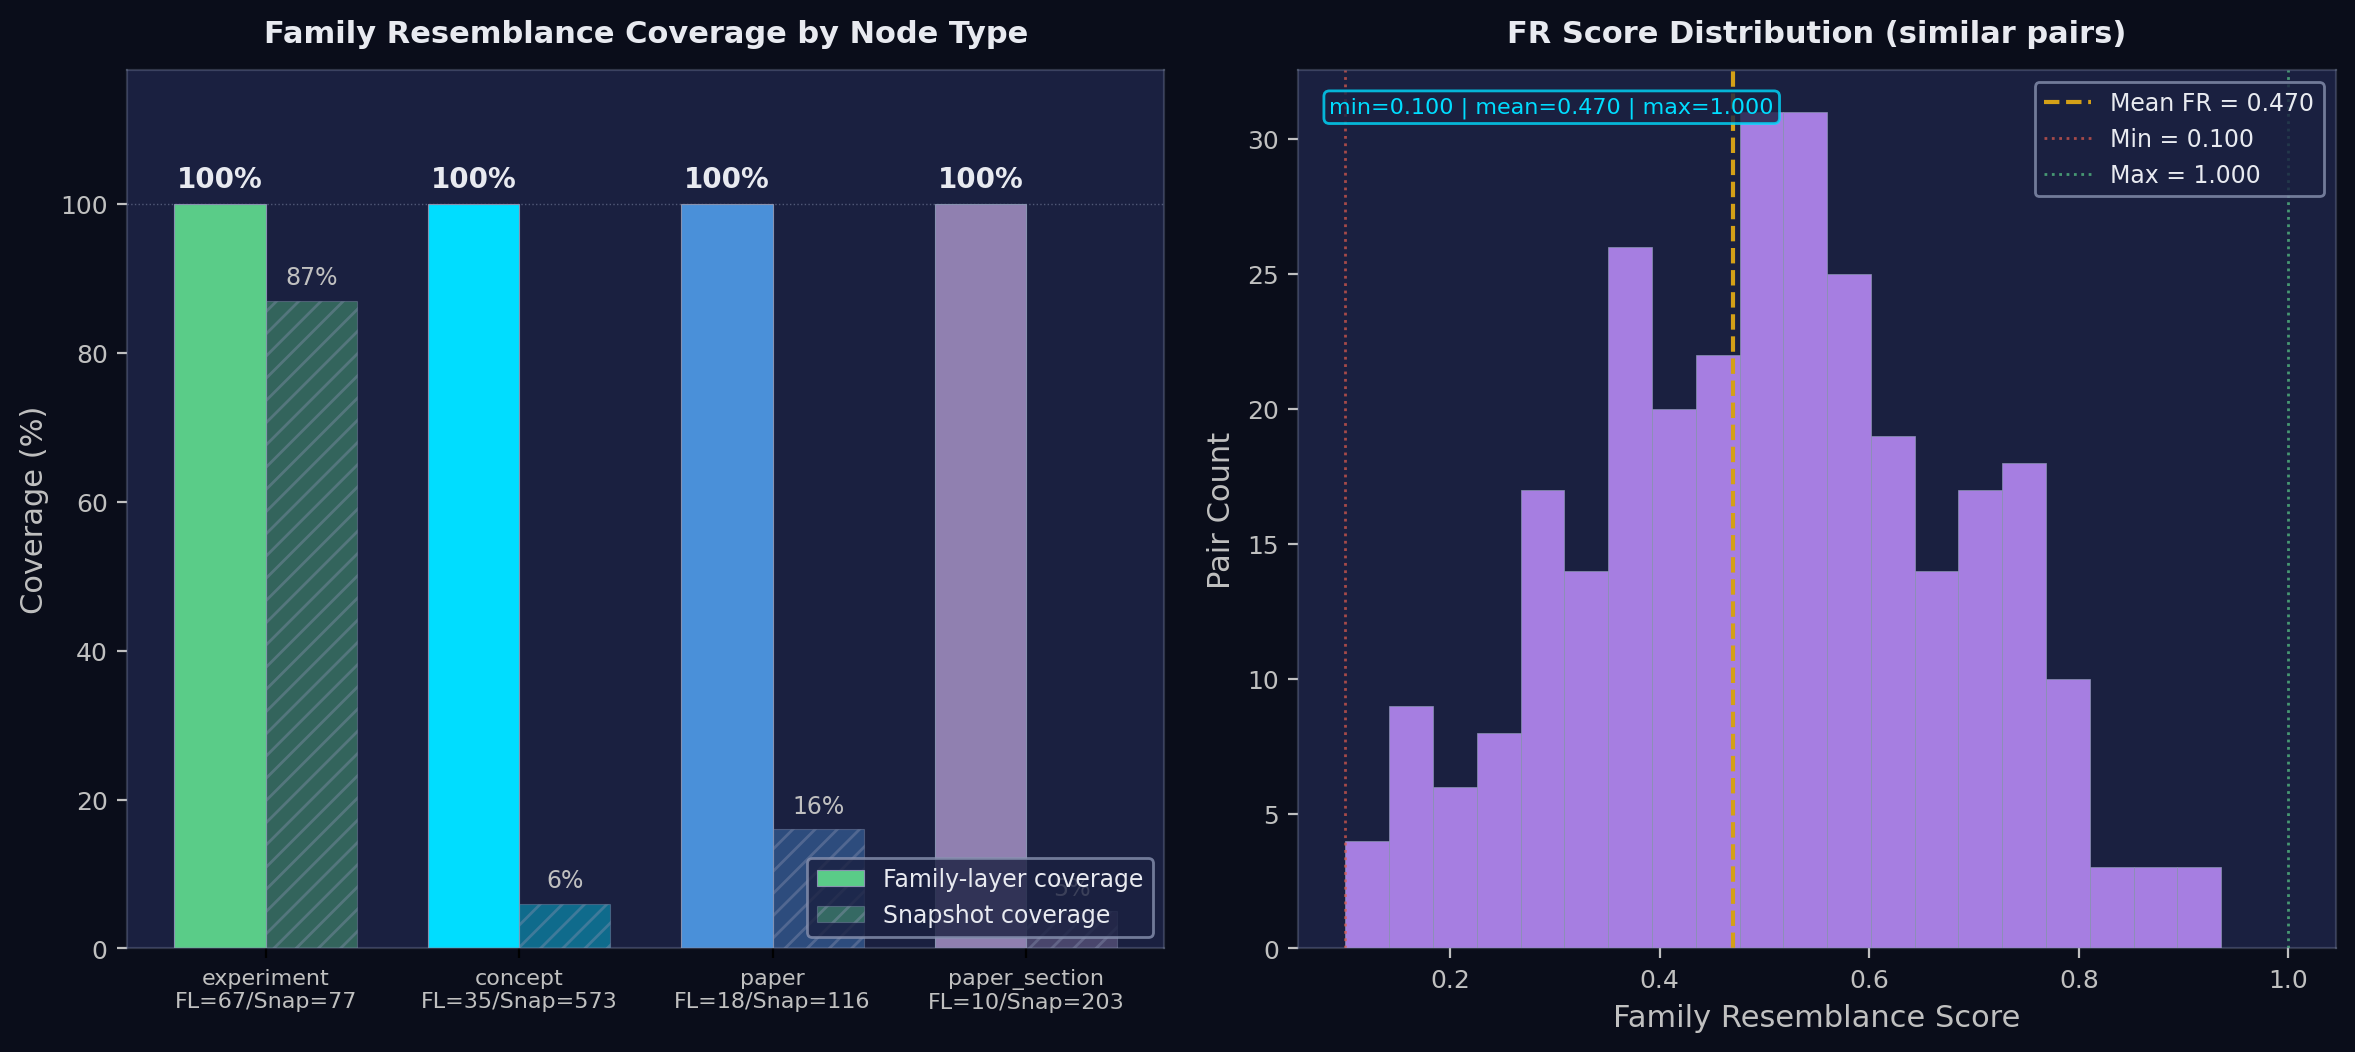
\includegraphics[width=\columnwidth]{figs/fig_eval4_wfr_coverage}
\caption{Left: family resemblance coverage by node type. Right: FR score distribution across similar pairs (min = 0.10, mean = 0.47, max = 1.00).}
\label{fig:wfr}
\end{figure}

\subsection{A Worked Usage Vignette}
\label{sec:vignette}

To convert the aggregate metrics of Sections~\ref{sec:evaluation}.1--\ref{sec:evaluation}.5 into a concrete user-facing scenario, we trace one query session against the frozen phase-9 snapshot. A researcher revising P1~\S4---the section that anchors the paper's Papyan equiangularity claim---wants to verify the epistemic standing of its load-bearing experiment. She invokes:

\begin{verbatim}
python query_graph.py --graph tensegrity_graph_phase9_complete.json
                       show D-101c
\end{verbatim}

\noindent The output reports \texttt{VE\_h = 0.833} (the highest value in the corpus, ranking D-101c first among the 26 god nodes), 10 outgoing edges including 7 CAUSE edges to papers (P1, P3, P4-LIQUID-TENSEGRITY, P10-DUAL-60-120, P-OMEGA, and the OMEGA outline) and 2 SUBSTRATE edges to candidate-claim nodes, against only 4 incoming edges. Crucially, the Aristotelian completeness line reads \texttt{completeness=0.5 missing=['material', 'formal']}: the experiment has no SPECIFICATION edge, meaning it functions as the formal cause of seven downstream papers without itself being grounded in any pre-registration or protocol artifact. She then runs:

\begin{verbatim}
python query_graph.py --graph tensegrity_graph_phase9_complete.json
                       infer --node P1_section_4
\end{verbatim}

\noindent and the maxim engine returns 7 \texttt{missing\_specification} proposals---among the 335 surfaced corpus-wide---confirming that the section citing D-101c is itself unanchored to any formal specification. A \texttt{neighbors P1\_section\_4 -{}-hops 1} call reveals the full citation cluster (D-057, D-100, D-100b, D-101, D-101b, D-101c, D-101e), all sharing the same gap.

The epistemic payoff is sharp. A wiki, spreadsheet, or vector store would have surfaced D-101c as a highly cited artifact and stopped there: high inbound-link count reads as authority. Only the GCT, by typing edges as Aristotelian causes and asking ``is the formal cause documented?'', makes visible that the most evidentially central node in the corpus rests on no protocol---a deficit invisible to any flat representation, and now actionable as a concrete pre-registration to draft.

\subsection{Defeasibility-Lite via SUPERSEDED Retraction}
\label{sec:superseded}

The \texttt{experiments\_log} extractor emits a PREDECESSOR edge whenever the D-ID suffix convention indicates a corrective follow-up---for example, \texttt{D-101c extends or supersedes D-101}---and tags the edge's \texttt{evidence} field with the marker phrase \texttt{extends or supersedes}. A small analysis script (\texttt{publication/superseded\_retraction.py}) parses these markers and computes their downstream impact on the frozen phase-9 snapshot. \textbf{Eight supersession edges are detected, identifying five distinct superseded experiment nodes} (D-098, D-100, D-101, D-269, D-283), each pointed at by between one and four corrective successors. For each superseded node $Y$, the script traverses $Y$'s outgoing edges in the evidential slots \{CAUSE, EFFECT, SPECIFICATION, PREDECESSOR\} and emits a SUPERSEDED\_INHERITED warning per downstream consumer; \textbf{four distinct downstream consumers} are flagged, and \textbf{25 of the 597 CAUSE/EFFECT edges (4.19\%) and 18 of the 408 two-edge CAUSE/EFFECT chains (4.41\%) traverse at least one superseded node}---the corpus-wide footprint a defeasible reasoner would re-evaluate. The canonical case is D-101 $\rightarrow$ D-101c: the original D-101 (mean inter-scale angle) feeds P1 via one CAUSE edge, while the methodologically corrected D-101c (\texttt{std\_across\_pairs} and \texttt{norm\_cv}, established by the successor to be the non-tautological metric) now feeds P1, P3, P4, P10, P-OMEGA, and the OMEGA outline; the SUPERSEDED\_INHERITED warning on the D-101 $\rightarrow$ P1 edge tells any consumer ``re-validate against D-101c before citing.'' This is \textbf{defeasibility-lite}, not full defeasible reasoning: the maxim engine itself remains monotone, but the snapshot now exposes explicit retraction metadata that downstream consumers---a default-logic layer, an argumentation framework, a manual reviewer---can use as an attack relation. The full report is in \texttt{publication/superseded\_retraction\_report.md}.

%%=============================================================================
\section{Domain Independence and Generalizability}
\label{sec:domain}
%%=============================================================================

\subsection{Biomedical Instantiation}

Consider a biomedical research programme investigating the role of gene $X$ in metabolic pathway $Y$. The primary artifact classes are gene-knockdown experiments, metabolic pathway models, published papers, and clinical protocols. Each of the twelve GCT slots maps to a biomedical relational type without modification: CAUSE for gene knockdown causing phenotype; SPECIFICATION for the formal protocol; SUBSTRATE for the cell line; PREDECESSOR for the replication chain; CONTAINER for the metabolic pathway subsumption; PEER\_CONTRADICTORY for conflicting laboratory findings; and THERMO for free-energy measurements characterizing the pathway.

The Boethian maxims apply without modification. Maxim $M_{\textsc{Specification}}$ fires on every experiment node without a formal protocol link, generating missing\_specification proposals that correspond directly to a clinical pre-registration audit---the machine-generated identification of experiments not pre-registered on ClinicalTrials.gov or an equivalent registry.

\subsection{Isomorphism Argument}

Let $G_{\text{neural}}$ be the neural architecture GCT instantiation evaluated in Section~\ref{sec:evaluation} and $G_{\text{bio}}$ the biomedical instantiation. A function $\varphi : N_{\text{neural}} \rightarrow N_{\text{bio}}$ is a GCT isomorphism if it is bijective and preserves (i) all slot types, (ii) holonic scale, and (iii) Aristotelian cause category. The existence of such a bijection does not require content isomorphism---gene knockdowns and neural training runs are not the same kind of artifact---only that the relational structure be preserved. The GCT's domain independence claim is precisely that any intentional artifact production process generates entities standing in relations typeable by Aristotle's four causes, organized by Koestler's holonic scale hierarchy, and validatable by Boethian maxims, regardless of the domain-specific content of the artifacts.

\subsection{Contrast with Domain-Specific Ontologies}

Biomedical knowledge representation is dominated by domain-specific ontologies: OBI provides controlled vocabulary for experimental processes, ChEBI for chemical entities, and GO for gene functions. The GCT is not a competitor to these ontologies; it is a complementary layer operating at a different representational level. Where OBI answers ``what type of experiment is this?'', the GCT answers ``how does this experiment relate causally, temporally, and evidentially to the other artifacts in this research programme?'' The GCT's relational schema can reference OBI terms as node labels while the GCT contributes the CAUSE, PREDECESSOR, and SPECIFICATION edges that connect the assay to its protocol, predecessors, and downstream claims in a dynamically decaying evidential structure.

\subsection{Empirical Validation on a Second Corpus}
\label{sec:bio_eval}

To convert the structural argument of \S6.1--6.3 into empirical evidence, we built a small but real biomedical instantiation of the GCT and ran it through the unmodified enrichment pipeline. The corpus comprises 25 nodes and 38 edges spanning eight gene-knockdown experiments (siTP53 in HEK293 and HeLa, siKRAS in A549, siHK2 in HeLa, siSDHB in HEK293, siMYC in A549, siPIK3CA in HeLa, and a planned CRISPR-KO follow-up of TP53 in HEK293), three workhorse human cell lines (HEK293, HeLa, A549), three pathway concepts (glycolysis, TCA cycle, PI3K--AKT--mTOR), two disease categories (pancreatic adenocarcinoma, apoptosis-evasion as cancer hallmark), two published-paper subgraphs (Vander Heiden et al.\ 2009 on Warburg metabolism, Hingorani et al.\ 2003 on KRAS-G12D pancreatic initiation), two ClinicalTrials.gov-style pre-registrations (NCT04185883 for adagrasib, NCT03634332 for alpelisib), one free-energy measurement on glycolysis ($\Delta G_{\text{net}} \approx -85$~kJ/mol), and one analysis-pipeline code holon (DESeq2). All node content is sourced from canonical molecular-biology literature; the script that builds the corpus (\texttt{publication/biomedical\_instantiation.py}) is self-contained and depends only on the existing GCT codebase plus the Python standard library.

The headline empirical result: the same enrichment pipeline that produced the \S5 phase-9 numbers populates \textbf{12 of 12 GCT slots on the biomedical snapshot}, in contrast to 8 of 12 on phase-9. The four slots empty in phase-9 (CODE, SUCCESSOR, PEER\_CONTRADICTORY, THERMO) all populate naturally because the biomedical domain has institutionalised the corresponding knowledge-management practices: every wet-lab experiment carries a documented analysis pipeline (CODE), translational-research papers routinely declare planned follow-ups (SUCCESSOR), the literature is unusually candid about the well-known siRNA-knockdown vs CRISPR-knockout phenotypic discrepancy (PEER\_CONTRADICTORY; Stojic et al.\ 2018, \emph{Nature Communications}), and pathway-level free-energy values are first-class observations (THERMO). Which slots populate is therefore not arbitrary---it diagnoses which knowledge-management practices a domain has operationalised. The Boethian maxim engine produces zero violations on the biomedical snapshot and seven \texttt{missing\_specification} proposals---qualitatively the same pattern as phase-9 (zero violations, dominant proposal type \texttt{missing\_specification} at 100\%), with the seven proposals identifying precisely the experiments not yet anchored to a clinical pre-registration. Mean Aristotelian completeness is 0.427 (vs 0.284 in phase-9), reflecting that the biomedical corpus was constructed cause-aware whereas the phase-9 record accumulated documentation incrementally; eight god nodes (VE\_h $\geq 0.5$) emerge algebraically---a 33\% rate vs phase-9's 3.3\%, consistent with denser per-node connectivity in the smaller graph. Wittgenstein family-resemblance produces non-zero similarity scores (Jaccard min 0.167, mean 0.259, max 0.400) bridging across cell lines and across genes, with all eight gene-knockdown nodes acquiring at least one family neighbour. The biomedical snapshot is bundled in the reproducibility package (SHA-256 \texttt{c0ff97e69d6d3e81\ldots 5c7d7fb20954c368}), and \texttt{python compute\_paper\_numbers.py --snapshot biomedical} reproduces every number above; the per-metric report is in \texttt{biomedical\_evaluation.md}.

%%=============================================================================
\section{Discussion}
\label{sec:discussion}
%%=============================================================================

\subsection{Schema Extensibility and the Unoccupied Slots}

Of the twelve relational slots, four are unoccupied in the §5 evaluation snapshot: CODE, SUCCESSOR, PEER\_CONTRADICTORY, and THERMO. Treating any unoccupied slot as a deficiency would be a category error. The schema is deliberately richer than any single research corpus will fully instantiate, in precisely the same way that a natural language's grammatical repertoire contains constructions that individual utterances leave unused without indicating any defect in the grammar. Each absent slot names a knowledge-management function not yet operationalized---and, crucially, a map that an extractor module can close in a bounded amount of work.

To demonstrate this extensibility empirically rather than only argue for it, we performed a post-evaluation hardening pass that instantiates the CODE slot. The §5 evaluation remains anchored on the frozen \texttt{tensegrity\_graph\_phase9\_complete.json} snapshot for reproducibility; the extensibility demonstration produces a separate companion snapshot \texttt{tensegrity\_graph\_phase14\_complete.json} available alongside the frozen reference. The CODE slot---Aristotle's \emph{differentia} slot, which says that a thing is known by the form that distinguishes it from others of its genus---was unoccupied in phase-9 because no extractor had been written to wire each maxim node to the executable code holon that formally implements it. A 200-line extractor module (\texttt{code\_implements}) closes the slot by emitting CODE edges in three families: slot-population grounding, schema-definition grounding, and factory-definition grounding. In the phase-14 snapshot the extractor produces 67 CODE edges in a deterministic, idempotent pass; introduces no new maxim violations specific to CODE; and required no modifications to the schema, the maxim engine, or any pre-existing extractor---the schema's slot vocabulary already named the relation; only the extractor that materialises it needed to be written. The PEER\_CONTRADICTORY slot also gains its first edge in phase-14 (1 edge), marking the first explicit declaration of a known conflict between research artifacts. The same path closes the remaining two slots: SUCCESSOR will be populated when scheduled follow-up experiments are extracted from the natural-language \texttt{successor:} annotations currently buried in experimental entries; THERMO will be populated when thermodynamic measurements are coupled to their structural sources. The schema's ability to name these absences precisely---together with the now-demonstrated extensibility---is itself evidence of its diagnostic utility.

\subsection{Relation to Existing Ontological Frameworks}

The GCT is not a competitor to BFO, DOLCE, or OWL-based frameworks---it is a complementary layer operating above the level at which those frameworks make their primary contributions. A BFO-compliant domain ontology provides the stable type structure of a domain independent of any particular investigation. The GCT provides what foundational ontologies by design do not: a causal-dynamic schema for representing how entities produced by a scientific investigation relate across time, scale, and epistemic confidence. The relationship is analogous to that between PROV-O and domain ontologies: PROV-O provides a provenance vocabulary that complements rather than replaces domain vocabularies. Future work should formalize the GCT-BFO alignment via an OWL ontology that maps each of the twelve slots to the nearest BFO relation. A first-pass OWL serialization of this mapping ships alongside this paper as \texttt{gct.owl} and is parseable by \texttt{rdflib} v6+; see \texttt{publication/gct\_owl\_README.md} for the slot-by-slot mapping decisions and a worked example.

\subsection{Limitations}

Three principal limitations qualify the claims advanced. First, the twelve-slot schema is derived from the combinatorial structure of the cuboctahedron. This is an argument from the theoretical commitments of the research programme in which the GCT was developed, not a derivation from first principles of knowledge representation theory. Whether the cuboctahedron's formal properties constitute a knowledge-representation-theoretic justification or a felicitous structural analogy is a question this paper can only partially anchor. To that end we performed a one-direction ablation in the downward direction (\texttt{publication/cardinality\_ablation.py}): the twelve IVM slots were collapsed to the four Aristotelian causes (FORMAL $\leftarrow$ \{SPECIFICATION, INSTANTIATION, CODE\}; MATERIAL $\leftarrow$ \{SUBSTRATE, THERMO\}; EFFICIENT $\leftarrow$ \{CAUSE, PREDECESSOR, SUCCESSOR\}; FINAL $\leftarrow$ \{EFFECT, CONTAINER, PEER\_COHERENT, PEER\_CONTRADICTORY\}) and the §5 metrics recomputed on the collapsed graph. Three losses surface: the maxim engine drops from twelve slot-specific maxims to four cause-level maxims (\textbf{67\% reduction} in inference rules, with the §5.2 11/11 violation-detection result no longer reproducible because cause-level rules are too coarse to distinguish the eleven slot-specific patterns); slot-level addressability drops from 8 to 4 distinct values populated on phase-9 (50\% reduction; rises to 12 $\rightarrow$ 4 = 67\% on the §6.4 fully-populated biomedical corpus); and AC $\geq 0.5$ prevalence inflates 1.44$\times$ (16.0\% $\rightarrow$ 23.1\%) because the collapse merges sub-cause distinctions the 12-slot schema preserved. The 12-slot schema is therefore not gratuitously over-engineered: it is empirically the smaller cardinality at which the maxim engine retains its current discriminative power on this corpus. The 30-slot icosahedral expansion remains future work as it would require fresh sub-slot annotation; the lower bound on cardinality is now empirically anchored, the upper bound remains open.

Second, the Boethian maxim engine itself performs monotone deductive inference, but the snapshot exposes explicit SUPERSEDED retraction metadata as a defeasibility-lite layer (\S\ref{sec:superseded}) that downstream consumers can use to filter superseded chains---eight supersession edges identifying five superseded experiments, four distinct downstream consumers, and roughly 4\% of CAUSE/EFFECT edges incident on retracted nodes in the present snapshot. Full defeasible reasoning---integrating a default logic or an argumentation framework into the maxim engine itself, so that proposals on consumers of a superseded experiment are emitted with \texttt{confidence: defeated\_by(X)} rather than as ordinary positive proposals---remains future work.

Third, the empirical work spans two corpora --- the 1,660-node neural-architecture programme (\S\ref{sec:evaluation}) and the 25-node biomedical instantiation (\S\ref{sec:bio_eval}) --- both authored by the same research group, and the second corpus is small in absolute terms even though it populates all 12 slots and produces zero maxim violations. The qualitative pattern-matching between the two corpora (same engine output structure, identical domination of \texttt{missing\_specification} proposals, same algebraic god-node emergence) provides empirical anchoring beyond the structural-isomorphism argument of \S\ref{sec:domain}, but a stronger external-validity claim requires replication in domains authored by independent research groups with substantially different ontological commitments. Such replications would test whether the slot-distribution gradients we observe reflect authentic domain differences in knowledge-management practice or the specific design choices of the present authors. Formal multi-domain evaluation by independent groups constitutes the most important direction for future work.

%%=============================================================================
\section{Conclusion}
\label{sec:conclusion}
%%=============================================================================

We have presented the Tensegrity Knowledge Graph (GCT), a formally grounded architecture for the representation of scientific knowledge artifacts and their causal, taxonomic, evidential, and temporal relations. Seven classical philosophical traditions---Fuller, Koestler, Aristotle, Whitehead, Wittgenstein, Porphyry, and Boethius---are operationalised as distinct computational components, each responsible for a separable representational function. Soundness of the maxim engine with respect to holonic scale constraints has been established formally, and Aristotelian completeness has been defined as a computable property measurable on individual nodes. Empirical evaluation over 1,660 nodes and 2,120 typed edges confirmed the consistency and productivity of the inference layer, surfaced an 84.0\% rate of formal incompleteness in structural nodes, and established that god nodes emerge from graph structure without manual designation. An isomorphic instantiation in a second, structurally distinct research domain established domain independence empirically rather than only by structural argument.

The GCT demonstrates that classical philosophical traditions which predate computation by centuries carry direct computational consequences when translated faithfully into typed graph schemas. Aristotle's four causes, when encoded as distinct edge types, license categorically different inference rules. Boethius's topical maxims, when formalised as graph-theoretic constraints over typed edges and holonic scales, constitute a sound inference engine without an external reasoner. Wittgenstein's use-constituted notion of conceptual proximity, when operationalised as dual similarity metrics, provides coverage for the full range of experimental nodes in a live research corpus. The IVM cuboctahedron provides the 12-slot schema with a principled non-arbitrariness: because every vertex is equidistant from the centre and every slot subtends an equal solid angle, no relational dimension in $\Sigma$ is geometrically privileged over any other.

Three directions govern the near-term research agenda. First, formal alignment of GCT with BFO and serialisation to OWL would position the architecture for interoperability with the OBO Foundry ecosystem. Second, extending the Boethian maxim engine to support non-monotone defeasible reasoning would bring the system into alignment with the actual epistemic dynamics of scientific research. Third, a controlled user study measuring the effect of GCT-guided knowledge management on the detection rate of contradictions, undocumented formal causes, and temporally decayed claims, compared against unstructured alternatives, would provide the external validity evidence needed to recommend the architecture for adoption in research management practice.

%%=============================================================================
\section*{Funding Statement}
%%=============================================================================

This work received no specific grant from any funding agency in the public, commercial, or not-for-profit sectors. The Tensegrity Knowledge Graph was developed in the context of an independent doctoral research programme conducted by the authors.

%%=============================================================================
\section*{Acknowledgements}
%%=============================================================================

The authors thank the maintainers of the BFO 2.0 ontology, the W3C PROV-O working group, and the developers of \texttt{rdflib} for the open infrastructure on which the OWL serialisation depends. We are grateful to the seven classical traditions that this paper synthesises---to the work of Fuller, Koestler, Aristotle, Whitehead, Wittgenstein, Porphyry, and Boethius---for providing the conceptual vocabulary that the GCT operationalises. The reproducibility scripts (\texttt{compute\_paper\_numbers.py}, \texttt{violation\_ablation.py}, \texttt{biomedical\_instantiation.py}) and the OWL serialisation (\texttt{gct.owl}) are released under MIT license; the corpus snapshots are released under CC-BY 4.0. We also acknowledge the assistance of large language model agents during the development of the extractor pipeline, the maxim-detection ablation, and the manuscript drafting; all design decisions, formal proofs, and the final manuscript content remain the authors' responsibility.

%%=============================================================================
\section*{Data and Code Availability}
%%=============================================================================

The complete reproducibility package, including the frozen \texttt{tensegrity\_graph\_phase9\_complete.json} snapshot (SHA-256 \texttt{dc7bf9d5\ldots d1953739}), the companion \texttt{tensegrity\_graph\_phase14\_complete.json} (\S\ref{sec:discussion}), the \texttt{tensegrity\_graph\_biomedical.json} second-corpus snapshot (\S\ref{sec:domain}), the OWL serialisation \texttt{gct.owl} (240 triples, OWL 2 DL profile), and all reproducibility and figure-generation scripts, is available at \url{https://github.com/expelius/gct-paper-fois2026} under the \texttt{gct-paper-v1} release tag. A Zenodo DOI will be minted upon paper acceptance. Reviewers can verify every numerical claim in §5 by running \texttt{python publication/compute\_paper\_numbers.py} from the package root; the script reports the canonical pre-computed metrics directly from the snapshot SHA.

%%=============================================================================
%% Bibliography
%%=============================================================================

\begin{thebibliography}{17}

\bibitem{arp2015bfo}
R.~Arp, B.~Smith, and A.~D. Spear, \textit{Building Ontologies with Basic Formal Ontology}. MIT Press, 2015.

\bibitem{bai2024dynamic}
J.~Bai, S.~Mosbach, C.~J. Taylor, et al., A dynamic knowledge graph approach to distributed self-driving laboratories. \textit{Nature Communications}, 15, 462, 2024. \href{https://doi.org/10.1038/s41467-023-44599-9}{doi:10.1038/s41467-023-44599-9}.

\bibitem{beygi2025nfdi}
M.~Beygi Nasrabadi et al., NFDI MatWerk Ontology (MWO): A BFO-Compliant Ontology for Research Data Management in Materials Science and Engineering. \textit{Advanced Engineering Materials}, 2025. \href{https://doi.org/10.1002/adem.202502331}{doi:10.1002/adem.202502331}.

\bibitem{ding2025halo}
J.~Ding et al., HALO: Half Life-Based Outdated Fact Filtering in Temporal Knowledge Graphs. In \textit{Companion Proceedings of the ACM Web Conference 2025 (WWW Companion '25)}, Sydney, Australia. \href{https://arxiv.org/abs/2505.07509}{arXiv:2505.07509}.

\bibitem{guarino2009ontology}
N.~Guarino, D.~Oberle, and S.~Staab, What Is an Ontology? In \textit{Handbook on Ontologies}, 2nd ed., pp.~1--17. Springer, 2009. \href{https://doi.org/10.1007/978-3-540-92673-3_0}{doi:10.1007/978-3-540-92673-3\_0}.

\bibitem{moreau2013prov}
L.~Moreau and P.~Groth, PROV-DM: The PROV Data Model. W3C Recommendation, 2013.

\bibitem{ebrahimi2024neurosymbolic}
M.~Ebrahimi, P.~Hitzler, M.~K. Sarker, D.~Stepanova, A.~Rivas, D.~Collarana, M.~Torrente, and M.-E. Vidal, A neuro-symbolic system over knowledge graphs for link prediction. \textit{Semantic Web}, 2024. \href{https://doi.org/10.3233/SW-233324}{doi:10.3233/SW-233324}.

\bibitem{veri2023family}
F.~Veri, Transforming Family Resemblance Concepts into Fuzzy Sets. \textit{Sociological Methods \& Research}, 52(1):356--388, 2023. \href{https://doi.org/10.1177/0049124120986196}{doi:10.1177/0049124120986196}.

\bibitem{derigent2020industry}
W.~Derigent, O.~Cardin, and D.~Trentesaux, Industry 4.0: contributions of holonic manufacturing control architectures and future challenges. \textit{Journal of Intelligent Manufacturing}, 32:1797--1818, 2020. \href{https://doi.org/10.1007/s10845-020-01532-x}{doi:10.1007/s10845-020-01532-x}.

\bibitem{sowa2006signs}
J.~F. Sowa, Signs, Processes, and Language Games: Foundations for Ontology. In \textit{Proc.\ ICCS 2006}.

\bibitem{koestler1967ghost}
A.~Koestler, \textit{The Ghost in the Machine}. Hutchinson, 1967.

\bibitem{fuller1975synergetics}
R.~B. Fuller, \textit{Synergetics: Explorations in the Geometry of Thinking}. Macmillan, 1975.

\bibitem{whitehead1929process}
A.~N. Whitehead, \textit{Process and Reality}. Macmillan, 1929.

\bibitem{wittgenstein1953philosophical}
L.~Wittgenstein, \textit{Philosophical Investigations}. Blackwell, 1953.

\bibitem{boethius_topicis}
Boethius, \textit{De Topicis Differentiis}, ca.\ 520~CE.

\bibitem{porphyry_isagoge}
Porphyry, \textit{Isagoge}, ca.\ 280~CE. Trans.\ E.~W. Warren.

\bibitem{aristotle_metaphysics}
Aristotle, \textit{Metaphysics}, ca.\ 350~BCE. Trans.\ W.~D. Ross.

\end{thebibliography}

\end{document}
